%%
%% Автоматизированная разработка програмно-аппаратного комплекса <<цифровые часы с будильником>>
%%

\documentclass[russian,utf8,pointsection]{eskdtext}
\usepackage[utf8]{inputenc}
\usepackage{eskdchngsheet}

\usepackage[ unicode ]{ hyperref }
\usepackage{amstext}
\usepackage{ amsmath }
\usepackage{ listings }
\graphicspath{{/Users/zolkko/Projects/zolkko-alarm/doc/imgs/}}

\ESKDdepartment{Федеральное агентство по образованиюГосударственное образовательное учреждениеВысшего профессионального образования<<Воронежский государственный технический университет>>(гоувпо <<ВГТУ>>)}
\ESKDcompany{}
\ESKDclassCode{31 1398}
\ESKDdocName{Пояснительная записка}
\ESKDsignature{TODO: ШИФР}


%% Разработка програмно-аппаратного комплекса <<Будильник>>
\ESKDtitle{Отчт по преддипломной практике}

\ESKDauthor{Анисимов~А.~Н.}
\ESKDtitleApprovedBy{Руководитель}{Барабанов~В.~Ф.}
%%\ESKDtitleAgreedBy{XXX}{XXX~X.~X.}
\ESKDtitleDesignedBy{студент группы ВМ-072}{Анисимов А.Н.}
%%\ESKDtitleDesignedBy{XXX}{XXX~X.~X}




\begin{document}
\maketitle
%Задание на курсовой проект%Лист замечаний руководителя
\tableofcontents

\newpage
%!TEX root = /Users/zolkko/Projects/zolkko-alarm/doc/main.tex
\section*{Введение}
\addcontentsline{toc}{section}{Введение}
\begin{par}
На сегодняшний день при проектировании систем промышленной автоматизации и устройств
бытового применения, перед проектировщиками и разработчиками встают вопросы не только технического
характера, но и вопросы экономической целесообразности применения тех или иных решений.
То есть при их решении необходимо учитывать не только системные характеристики применяемых для
реализации конечных устройств технологий, но и искать компромис с их стоимостью. При этом
на конечную стоимость изделия будут влиять цена применённых схемотехнических решений,
время затраченное на проектирование и реализацию устройства, цена применяемых средства автоматизации
и цена специалистов проектировщиков и разработчиков.
\end{par}

\begin{par}
Немаловажным при проектировании устройств является учёт стремления
современной европейской культуры не только к открытым, но и полностью свободным системам,
зачастую обладающим более качественными системными и
потребительскими характеристиками и способствующими общему\\*
научно-техническому прогрессу \cite{lessing}.
\end{par}


В дипломном проекте рассмотрены современные методы и средства проектирования и разработки
программно-аппаратным комплексов на базе микроконтроллеров AVR компании Ateml. При этом
в процессе проектирования и разработки отдавалось предпочтение именно свободному или
доступному по цене программному и аппаратному обеспечению. В качестве примера разрабатывался
программно-аппаратный комплекс <<Универсальная система терморегулирования на базе
микроконтроллера AVR cемейства XMega>>. Таким образом в процессе выполнения дипломного проекта
стало возможным проведение анализа пригодности для практического применения свободного,
бесплатного и доступного по цене программного и аппаратного обеспечения для целей промышленного
производства.

Программный код написанный в процессе выполнения дипломного проекта использует большинство
внешней периферии микроконтроллера. Таким образом, сформированный программный код и электрическая
принципиальная схема, позволяют оценить преимущества и недостатки использования
микроконтроллеров AVR семейства XMega.

\newpage{}



%!TEX root = /Users/zolkko/Projects/zolkko-alarm/doc/main.tex
\section{Анализ современных систем автоматизированного проектирования про\-гра\-ммно\--аппа\-ра\-тных микроконтроллерных комплексов}

\subsection{Общие сведения о САПР}
\begin{par}
САПР --- Система автоматизированного проектирования --- автоматизированная система, реализующая
информационную технологию выполнения функций проектирования, представляет собой
организационно-техническую систему, предназначенную для автоматизации процесса проектирования,
состоящую из персонала и комплекса технических, программных и других средств
автоматизации его деятельности.
\end{par}

\begin{par}
На некотором этапе своего развития системы проектирования претерпели качественное изменение.
Оно было связано с тем, что САПР из набора каким-то образом связанных между собой прикладных
программ начали превращаться в мобильные и стройно организованные системы, способные к
настройке на особенности предметной области и на требования конечного пользователя,
допускающие расширение функциональных возможностей за счёт сравнительно несложного подключения
новых прикладных программных модулей и обеспечивающих поддержку групповой разработки сложных схем
коллективом проектировщиков.
\end{par}

\begin{par}
Особенное значение САПР приобрели в микроэлектронике, поскольку современная радиоэлектронная аппаратура базируется на применении сверхбольших
интегральных схем, разработка которых без применения САПР невозможна или крайне затруднительна.
\end{par}

\begin{par}
Специализированные САПР для разработки электронных устройств и печатных плат получили название
Electronic Design Automation - EDA, автоматизация проектирования электронных приборов.
Комплексы такого типа зачастую позволяют создавать принципиальные электрические схемы схемы с
помощью графического интерфейса, создавать и модифицировать  базу радиоэлектронных компонентов,
проверять целостность сигналов на ней и проводить аналоговое и цифровое моделирование
разрабатываемого устройства ещё на этапе проектирования.
\end{par}


\subsubsection{Обзор Electric VLSI}
\begin{par}
Electric VLSI --- cистема автоматизированного проектирования сверхбольших интегральных схем, используемая для разработки электрических схем и проектирования
топологии печатных плат и интегральных схем.
\end{par}
\begin{par}
Electric являлся open-source проектом, разработка
которого в течении многих лет поддерживалась\cite{electric} компанией Sun Microsystems,
а в настоящее время курируется компанией Oracle. \\*
Наиболее ценная встроенная в Electric возможность —-- это система привязок,
которая даёт возможность осуществлять проектирование сверху вниз с соблюдением целостности
всех соединений.
\end{par}

\subsubsection{Обзор Proteus VSM}
\begin{par}
Proteus VSM --- пакет программ для автоматизированного проектирования электронных схем.
    Разработка компании Labcenter Electronics.
\end{par}
\begin{par}
Proteus VSM сочитает в себе функциональность SPICE симуляции электронных цепей,
анимированные компоненты, модели микропроцессоров и средства симуляции сложных
микроконтроллерых решений. Это первая система сочетающая в себе все эти особенности
и позволяющая разработать и протестировать решение до создания прототипа устройства.
Такое тестирование осуществляется за счёт взаимодействия с отображаемыми и анимированными
виртуальными устройствами такими как свето-диоды, LCD, кнопки и переключатели.
При этом симуляция производится в режиме блиском к режиму реального времени.
Так производительности 1 ГГц Pentium III ЭВМ будет достаточно для симуляции работы
микропроцессора 8051 на частоте 12 МГц в режиме реального времени. Так же Proteus VSM
предоставляет экстенсивные средства отладки, включая точки останова, трассировку и вывод
значений  переменных микропрограмм как для машинных кодов, так и для языков высокого
уровня. Proteus VSM  включает несколько виртуальныхинструментов: осцилограф, логический
анализатор, генератор функций, генератор по шаблонам, виртуальный терминал, отладчики SPI
и I2C интерфейсов , а так же простые инструменты как вольтметр и амперметр, существенно
облегчающих анализ и отладку схемы.
\end{par}
\begin{par}
В дополнении к моделям микропроцессоров в Proteus VSM так же включена большая библиотека
стандартных пассивных и акивных моделей устройств.
\end{par}
\begin{par}
Пакет Proteus состоит из двух частей, двух подпрограмм: ISIS – программа синтеза и
моделирования непосредственно электронных схем и ARES – программа разработки печатных
плат.

\begin{figure}[h]
	\center{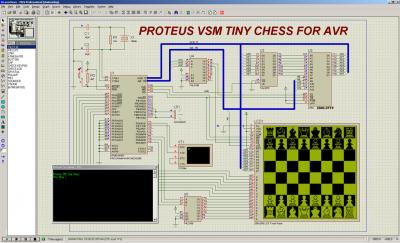
\includegraphics[bb=0 0 400 243, clip, scale=0.8]{proteus.png}}
	\caption{Главное окно программы Proteus ISIS}
	\label{img:proteus}
\end{figure}

\end{par}

\subsubsection{Обзор KiCAD}
\begin{par}
KiCad --- распространяемый по лицензии GNU General Public License программный
комплекс класса EDA с открытыми исходными текстами, предназначенный для разработки
электрических схем и печатных плат. \\*
Кроссплатформенность компонентов KiCad обеспечивается использованием библиотеки wxWidgets.
Поддерживаются операционные системы Linux, Windows NT 5.x, FreeBSD и Solaris.
\begin{figure}[h]
	\center{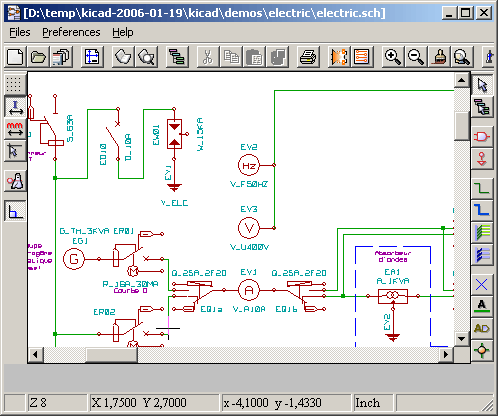
\includegraphics[bb=0 0 498 416, clip, scale=0.5]{kicad.png}}
	\caption{Главное окно программы KiCAD Eeschema}
	\label{img:kicad}
\end{figure}
\end{par}

\begin{par}
В состав KiCAD входят программы:
    \begin{itemize}
        \item{}kicad --— менеджер проектов;
        \item{}eeschema —-- редактор электрических схем (рис. \ref{img:kicad});
        \item{}встроенный редактор символов схем (библиотечных компонентов);
        \item{}pcbnew --— редактор печатных плат;
        \item{}встроенный редактор образов посадочных мест (библиотечных компонентов);
        \item{}3D Viewer --— 3D-просмотрщик печатных плат на базе OpenGL (часть pcbnew);
        \item{}gerbview --— просмотрщик файлов Gerber (фотошаблонов);
        \item{}cvpcb --— программа для выбора посадочных мест, соответствующих компонентам на схеме;
        \item{}wyoeditor --— текстовый редактор для просмотра отчетов.
    \end{itemize}
\end{par}


\subsubsection{Обзор gEDA}
\begin{par}
gEDA --- набор программного обеспечения для проектирования электронных устройств,
распространяемый по лицензии GPL. Включает в себя инструменты для редактирования
электрических схем, симуляции цифровых и аналоговых схем, трассировки печатных плат
и подготовки к производству. Проект изначально ориентирован на UNIX-совместимые
платформы, хотя некоторые программы, входящие в его состав, в настоящее время
портированы под ОС Windows\cite{geda}.
\end{par}
\begin{par}
В настоящее время пакет вполне пригоден для проектирования устройств среднего уровня
сложности и может быть полезен как студентам, любителям, так и профессиональным
разработчикам электронных устройств.
\end{par}
\begin{par}
За время существования проекта, к нему примкнуло несколько самостоятельных
узкоспециализированных проектов, которые теперь считаются частью gEDA, в
связи с чем оригинальный проект и его составные части стали называть
gEDA/gaf (gschem and friends) (рис. \ref{img:geda}).
\begin{figure}[h]
	\center{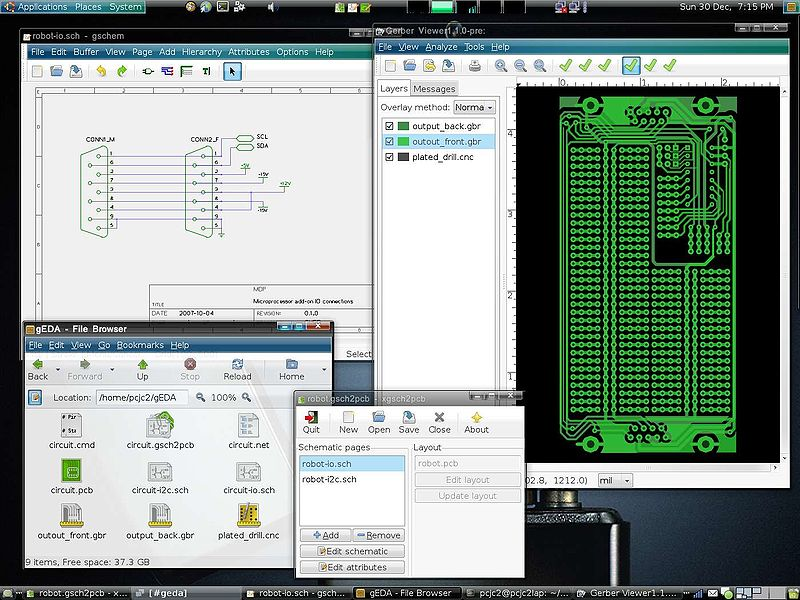
\includegraphics[bb=0 0 800 600, clip, scale=0.3]{geda.png}}
	\caption{gEDA}
	\label{img:geda}
\end{figure}
\end{par}

\subsubsection{Обзор Eagle EDA}
\begin{par}
EAGLE это лёгкий в использовании, но достаточной мощный EDA пакет, разрабатываемый немецкой компанией CadSoft.
В состам системы входят:
\begin{enumerate}
	\item{}Layout Editor --- пограмма для проектирования печатных плат (рис. \ref{img:eagle_brd}). 
		\begin{itemize}
			\item{}Максимальная рабочая поверхность 1.6 x 1.6м;
			\item{}разрешение - 1/10,000мм (0.1 микрон);
			\item{}до шестнадцати сигнальных слоёв;
			\item{}большая библиотека компонентов;
			\item{}copper pouring - области на печатной плате заполненные  медью, что часто используется для создания областей <<земли>> и уменьшения необходимого травильного вещества при производстве;
			\item{}встроенная ДРЦ проверка.
		\end{itemize}
        \begin{figure}[h]
            \center{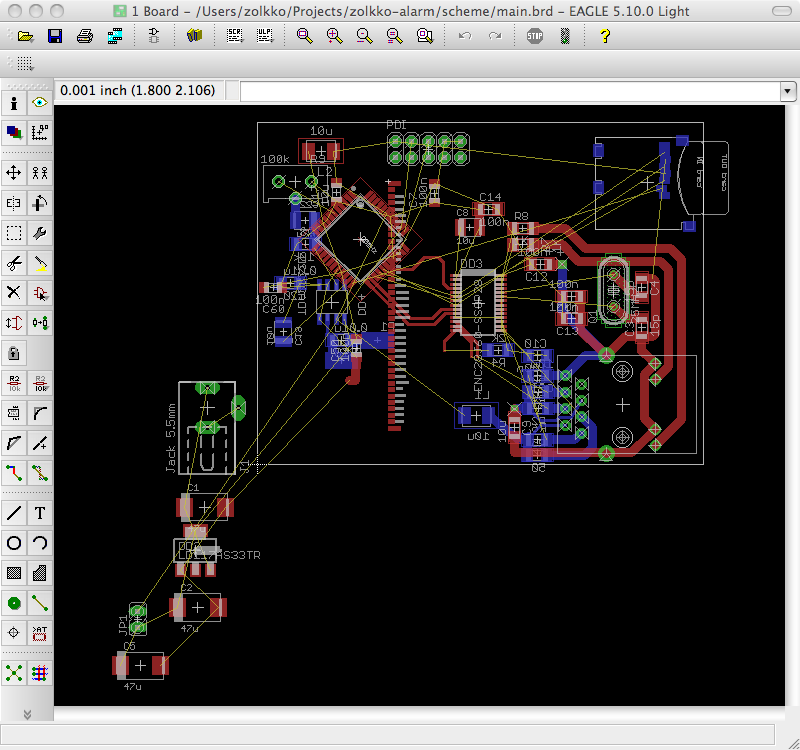
\includegraphics[bb=0 0 800 800, clip, scale=0.3]{eagle_brd.png}}
            \caption{Окно редактора печатных плат Eagle}
            \label{img:eagle_brd}
        \end{figure}

	
	\item{}Schematic Editor - программа для создания принципиальных электрических схем (рис. \ref{img:eagle_sch}).
		\begin{itemize}
			\item{}до 999 листов на одну схему;
			\item{}проверка эллектичских правил;
			\item{}обмен вентелей и пинов;
			\item{}возможность создания печатной платы из схемы одной командой.
		\end{itemize}
        \begin{figure}[h]
            \center{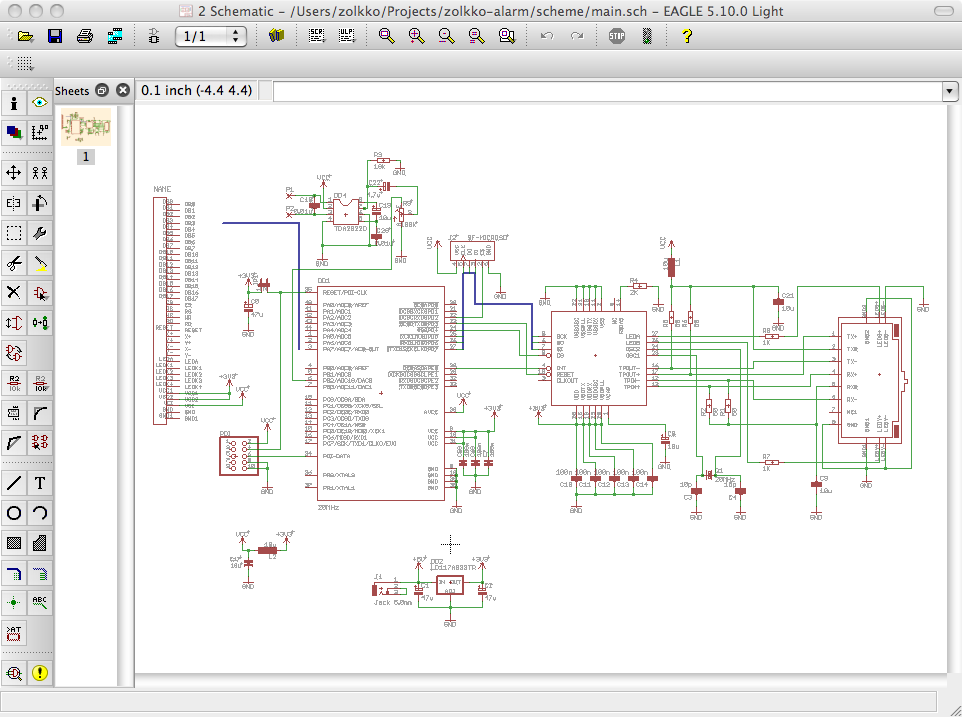
\includegraphics[bb=0 0 1010 730, clip, scale=0.3]{eagle_sch.png}}
            \caption{Окно редактора пренципиальных схем Eagle}
            \label{img:eagle_sch}
        \end{figure}
	\item{}Autorouter - программа автоматической трассировки.
		\begin{itemize}
			\item{}ripup-and-retry трассировщик - на первом проходе выполняется соединение абсолютно всех проводников без обращения внимания на возможные конфликты, заключающиеся в пересечении проводников на одном слое и нарушении зазоров. На каждом последующем проходе автотрассировщик пытается уменьшить количество конфликтов, разрывая и вновь прокладывая связи;
			\item{}до шестнадцати сигнальных слоёв;
			\item{}стратегия трассировки может быть подстроена заданием весовых коэфициентов.
		\end{itemize}
\end{enumerate}

Все эти программы встроены в один пользовательский интерфейс, таким образом нет необходимости в
предварительном конвертировании нет-листов.
\end{par}


\subsection{Обзор современных систем программирования микроконтроллеров}

Ведущими разработчиками 8/16 битных микроконтролеров на сегодняшний день
являются компании:
\begin{itemize}	
	\item{} Microchip Technology Inc. -- выпускающие микроконтроллеры семейства PIC и
		сигнальные микроконтроллеры dsPIC,
		получивших широкое распространение в странах серевной и южной америки.
		Отличительной особенностью PIC--контроллеров является хорошая преемственность
		различных семейств.
		8-битные микроконтроллеры представлены двумя базовыми архитектурами ядра:
		BASELINE и MID-RANGE. Основным инструментом разработки является среда программирования
		MPLab и набор компиляторов GCC.
	\item{} STMicroelectronics -- европейская компания, активно продвигающая свои 8 и 32
		разрядные микроконтроллеры на рынке. В качестве среды разработки предлагается
		использовать адаптированную версию набора компиляторов GCC.
	\item{} Texas Instruments --специализирующаяся на выпуске цифровых сигнальных процессоров
		и наиболее удачной линейки микроконтрллеров общего назначения MSP430.
	\item{} NXP Semiconductors -- производит 8 разрядные микроконтроллеры
			80C51: LPC900 и LPC700.
			Основным инструментом разработчика является адаптированная версия
			Keil PK51 Professional Developers Kit, предоставляющей инструменты для
			генерации программ для LPC, и включающая в себя среду разработки
			$\mu{}$Vision IDE, C51 ANSI C компилятор и A51 макро ассемблер, $\mu{}$Vision отладчик
			со встроенным симулятором ЦПУ и переферийных устройств. В комплект поставки
			среды так же входит внутрисхемный отладчик ISD51.			
	\item{} Freescale Semiconductor -- HC80, HC05, HC11.
	Эти микроконтроллеры используют расширенную архитектуру ЦПУ M68HC08.
	Основным иструментом разработки является CodeWarrior Development Studio, в поставку
	которой так же включается симулятор чипа и мастер автоматического генерирования
	кода ''Processor Expert''.
	\item{} Atmel Corporation -- выпускает микроконтроллеры AVR, основанные на ядре
	собственной разработки. Основное средство разработки -- AVR Studio. В начале 2011
	года компания прекратила поддержку старых версий AVR Studio 4 и AVR Studio 32,
	заместив их AVR Studio 5 -- средой разработки основанной на Microsoft Visual
	Studio Shell. В качестве компилатора выступает адаптированная версия GCC. Так
	же в комплекте среды разработки поставляется симулятор ЦПУ и переферии, и
	набор программного обеспечения ''AF''.
\end{itemize}

Таким образом, все лидирующие производители микроконтроллеров предоставляют
бесплатные системы программирования своих мкроконтроллеров.
Причём, можно отметить, что системы программирования либо основанны на коде 
набора компиляторов GNU GCC, либо в качестве стандартной среды разработки лицензируется
программное обеспечение других компаний. Во втором случае, зачастую, бесплатные
стандартные системы программирования обладают рядом ограничений, позволяющим только
опробовать демонстрационные проекты.

Однако, на рынке пристствует довольно большео число компаний специализирующихся
исключительно на создании систем программирования для встраиваемых систем. Лидером
в этой области является IAR Systems -- компания предоставляющая широчайший перечень компиляторов и стандартных библиотек для большого числа микроконтроллеров разных архитектур.
Их продукт IAR Embedded Workbench поддерживает следующие семейства микроконтроллеров:
\begin{itemize}
	\item{} 8051;
	\item{} ARM;
	\item{} Atmel AVR, AVR32;
	\item{} Freescale ColdFire, Freescale S08, Freescale HCS12;
	\item{} Maxim MAXQ;
	\item{} Microchip dsPIC/PIC24, PIC18;
	\item{} National CR16C;
	\item{} Renesas RL78, 78K, V850, H8, M16C, R8C, M32C, RX, R32C, SuperH;
	\item{} Samsung SAM8;
	\item{} STMicroelectronics STM8;
	\item{} TI MSP430.
\end{itemize}
Ещё одним интерестным продуктом этой компании является IAR visualState -- системе
программирования, автоматически генерирующей программный код на основе графически
заданного конечного автомата. При этом возможно проводить комдинированную разработку
программного обеспечения, когда часть кода программы генерируется автоматически, а часть
разрабатывается программистом.

\begin{figure}[h]
	\center{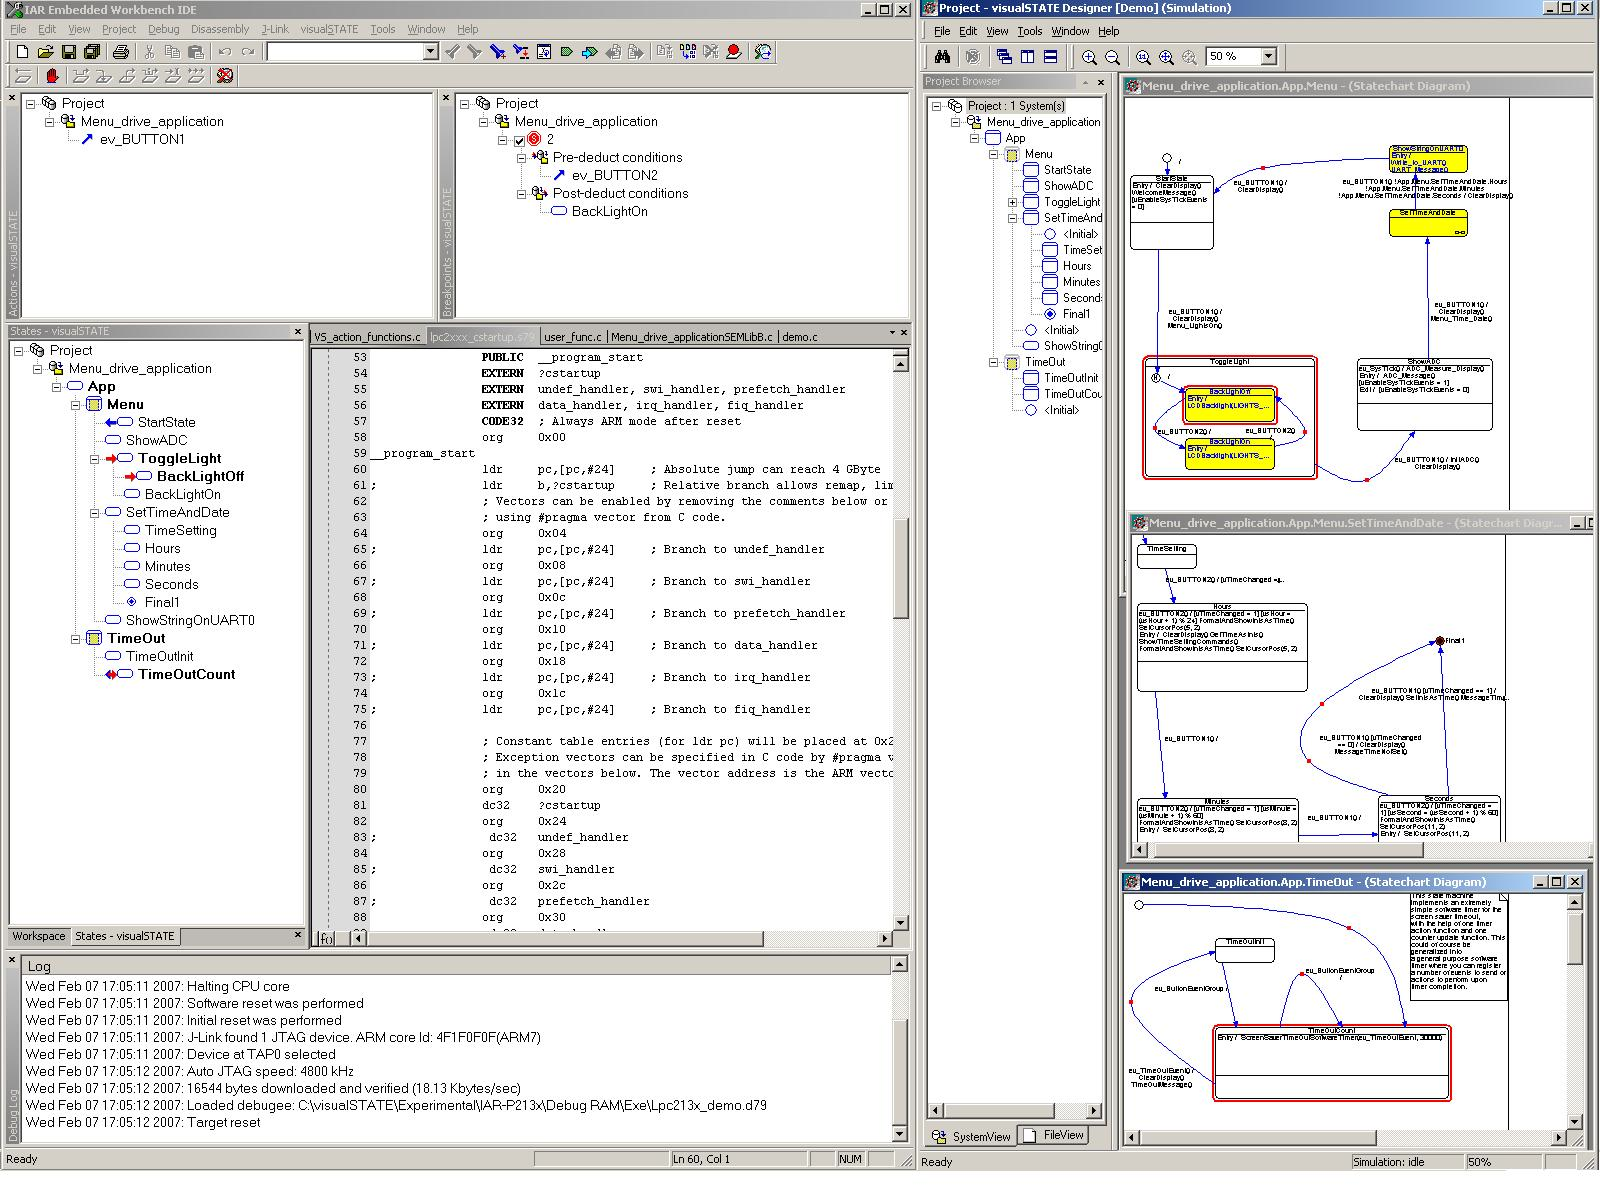
\includegraphics[bb=0 0 900 700, clip, scale=0.3]{iar_vis_state.png}}
	\caption{Среда разработки IAR visualSTATE}
	\label{img:iarVis}
\end{figure}

\newpage{}


%!TEX root = /Users/zolkko/Projects/zolkko-alarm/doc/main.tex
\section{Выбор инструментальных средств разработки микроконтроллерного программно-аппаратного комплекса}

\subsection{Выбор микроконтроллера}
Основными требованиями предъявляемыми мной к центральному вычислительному устройству
создаваемого устройства является:
\begin{itemize}
	\item{} невысокая стоимость;
	\item{} низкое энергопотребление;
	\item{} в число поддерживаемой переферии должен присутствовать ЦАП;
	\item{} аппаратная поддержка SPI;
	\item{} поддержка производителем этого рода устройств;
	\item{} доступность устройства;
	\item{} <<сильное>> сообщество разработчиков под эту архитектуру;
	\item{} наличие литературы и справочных материалов.
\end{itemize}


По всем этм пунктам идеально подходит микроконтрллер семейства XMega компании ATmel -- atxmega32a4.
Этот микроконтроллер полностью отвечает минимальным требованиям. В целях достижения максимальной
производительности и параллелизма у микроконтроллеров AVR используется
Гарвардская\\*
архитектура (рисунок \ref{img:avr_arch}) с отдельными памятью и шинами программ и данных. Инструкции,
хранящиеся в памяти программ, выполняются на одноуровневом конвейере. Это означает, что
во время выполнения одной инструкции выполняется предварительная выборка из памяти программ
следующей инструкции. Данная концепция делает возможным выполнение по одной инструкции за
каждый цикл синхронизации.

\begin{figure}[ht]
	\center{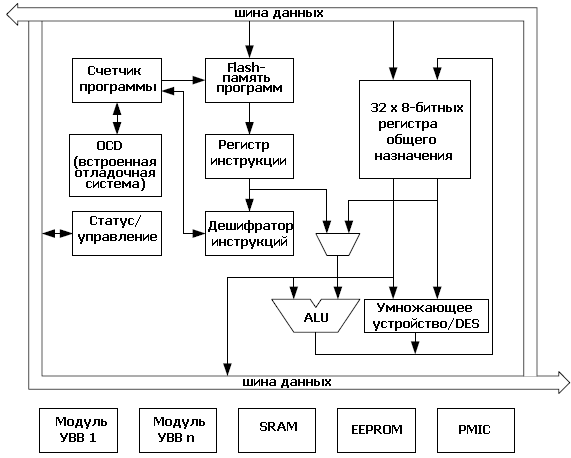
\includegraphics[bb=0 0 590 460, clip, scale=0.6]{avr_arch.png}}
	\caption{Архитектура AVR}
	\label{img:avr_arch}
\end{figure}


Так же в случае необходимости может быть заменён на более мощьный микроконтроллер того же семейства.
Для обеспечения этого функционала компания Atmel предприняла ряд шагов.

\begin{par}
    1. Была реорганизована область памяти, таким образом, чтобы все связанные между
            собой регистры располагались в памяти строго последовательно.
\end{par}
\begin{par}
    2. Была переписана стандартная библиотека C/C++, так чтобы обеспечивалась
            максимальная переносимость кода написанного для одного микроконтроллера
            на другой микроконтроллер того же семейства.
\end{par}

Микроконтроллеры серии XMega обладают следующими характеристиками:
\begin{itemize}
	\item{} 8/16-разрядное высокопроизводительное RISC ЦПУ AVR;
	\item{} 138 инструкций;
	\item{} аппаратное умножающее устройство;
	\item{} 32 8-битных регистра, напрямую подключенные к АЛУ
	\item{} прямая адресация до 16 Мбайт памяти программ и 16 Мбайт памяти данных;
	\item{} полная поддержка 16/24-битного доступа к 16/24-битным регистрам ввода-вывода;
	\item{} эффективная поддержка 8-, 16- и 32-битных арифметических инструкций;
	\item{} защита от изменения настроек критических функций системы.
\end{itemize}

Помимо этого, по сравнению с предыдущим семейством Mega \cite{avrref}, в микроконтроллеры семейства
XMega был внесен ряд значительных изменений.

\begin{par}
    1. Свехмалое энергопотребление обеспечиваемое технологией picoPower второго поколения.
    picoPower позволяет еще больше улучшить эффективность использования батарейного источника.
    То, что микроконтроллеры гарантируют нормальное функционирование при напряжении 1.6 В означает,
    что, например, в составе мобильных телефонов, они могут быть запитаны от стабилизированного
    источника напряжением 1.8В 10\%, тем самым, позволяя снизить себестоимость системы и увеличить
    длительность работы от батарейного источника. 
\end{par}

\begin{par}
    2. Event System -- позволяет организовать передачу данных между встроенными периферийными
    устройствами без вмешательства ЦПУ или использования ПДП.
    Этим гарантируется 100\% предсказуемость и малое время реагирования.
    До 8 одновременных событий или условий прерывания в периферийных устройствах могут автоматически
    инициировать действия в других периферийных устройствах \cite{avrxm}.
\end{par}

\begin{par}
    3. 12-разрядные АЦП и ЦАП. Для обеспечения высокоточной обработки аналоговых сигналов в состав 
    микроконтроллеров XMEGA интегрированы 12-битные преобразователи аналоговых сигналов. АЦП
    микроконтроллеров XMEGA могут достигать частоты преобразования до 2 МГц, что делает их самыми
	быстродействующими и точными на фоне АЦП обычных микроконтроллеров.
	Поскольку микроконтроллеры XMEGA также интегрируют два 12-битных ЦАП на частоту преобразования
	до 1 МГц и четыре усовершенствованных аналоговых компаратора, это делает их лидерами по
	степени интеграции компонентов для аналоговой обработки.
\end{par}

\begin{par}
   4. Расширена функциональность портов ввода-вывода общего назначения. Каждый из портов
    ввода-вывода может быть сконфигурирован как источник внешнего прерывания, при этом событие внешнего прерывания
    может минуюя ЦПУ запускать обработку данных используя модуль прямого доступа к памяти. \\*
    Новыми доступными состояниями портов ввода-вывода стали totem-pull, bus-keeper, wired-or, wired-and.
\end{par}


\subsection{Язык программирования микроконтроллера}
\begin{par}
Микропрограммы для микроконтроллеров XMega можно писать на нескольких языках программирования.
Сама компания Atmel предоставляет для программирования своих устройств два средства разработки:
	\begin{enumerate}
		\item{}AVR assembler -- язык низкого уровня, транслирует исходный код пользовательской
                программы в объектны и исполняемый код, его применение позволяет
                добиться от программы наибольшей производительности;
		\item{}AVR-GCC -- кодогенератор и набор дополнительных утилит для Gnu C Compiller от
                компании Atmel, активно поддерживаемый сообществом разработчиков, а так же
                входящий в комплект среды разработки AVR Studio, AVR32 Stdio и
                распростроняемый на правах свободного программного обеспечения, в состав
				которого входят компиляторы языка C и C++.
	\end{enumerate}
\end{par}

\begin{par}
В начале 2011 года компания предоставила новую версию своей интегрированной системы
разработки - AVR Studio 5. В отличии от предшественника, новая система позволяет разрабатывать
программное обеспечение для всех семейств микроконтроллеров AVR используюя единую среду разработки.
\end{par}

\begin{par}

\begin{figure}[ht]
	\center{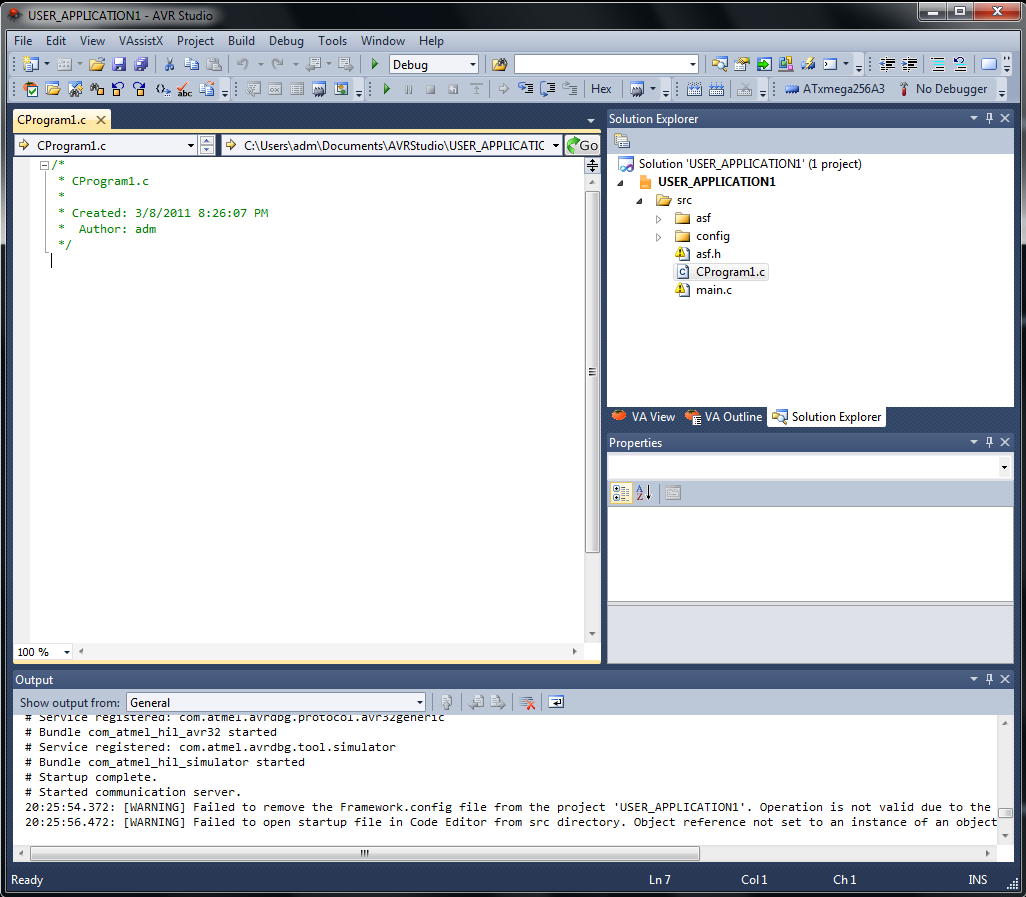
\includegraphics[bb=0 0 800 700, clip, scale=0.5]{avrstudio5.png}}
	\caption{AVR Studio 5}
	\label{img:avr_studio}
\end{figure}


Новая среда разработки AVR Studio 5 (рисунок \ref{img:avr_studio}) основана на базе лидирующего
продукта -- Microsoft Visual Studio.
И так же как и предшественники, новая версия AVR Studio 5  распространяется бесплатно.
В качестве компилятора и кодогенератора в AVR Studio 5 по прежнему используется AVR-GCC,
что позволяет продолжать использовать уже существующие наработки.
\end{par}

\begin{par}
Считается \cite{avrev}, что для разработки эффективного встраиваемого приложения для 8-битных микроконтрллеров
AVR наиболее целесообразно применять язык ассемблера или в случае, когда необходимо добиться
большей читаемости и поддерживаемости приложения -- язык С.
Однако, лидирующая группа японских производителей ЦПУ, возглавляемая NEC, Hitachi, Fujitsu и Toshiba,
разработала специализированных диалект языка C++ --- Embedded C++ (EC++), позволяющий применять
C++ для встраиваемых систем. Основная цель разработки --- перенос существующих методологий и шаблонов
программирования C++ в облать применения встраивамых систем.
При этом программы код генерируемых компиляторами EC++ может даже дать приемущества по сравлению
с языком C. Так как сама структура языка C++ позволяет минимизировать объём кода и одновременно
повышая его эффективность.
\end{par}

\begin{par}
Однако, при выборе в качестве языка программирования C++, из текущей реализации поставляемой с AVR-GCC,
необходимо учитывать некоторые её ограничения.
\end{par}

\begin{par}
 	1. В наборе компиляторов AVR-GCC отсутствует стандартная библиотека C++.
\end{par}

\begin{par}
	2. Необходимо помнить, что EC++ -- это только подмножество C++, по этому некоторые особенности языка были
        убраны из стандарта:
        \begin{itemize}
            \item{} множественное наследование;
            \item{} базовые виртульаные классы;
            \item{} информация времени исполнения;
            \item{} приведение типов (static\_cast, dynamic\_cast, reinterpret\_cast и const\_cast);
            \item{} квалификаторы типов;
            \item{} пространства имён;
            \item{} исключения;
            \item{} шаблоны.
        \end{itemize}
\end{par}



\subsection{Выбор языка программирования сетевого сервиса}

При проектировании сетевого сервиса от инструментального средства ожидается, чтобы оно
отвечало следующим требованиям \cite{technob}:

\begin{enumerate}
	\item{} инструментальное средство должно быть высокого уровня --- язык высокого уровня,
            освобождает разработчика от рутинной работы вроде ручного выделения и освобождения
            памяти, и позволяет ему сфокусироваться на оперировании абстракциями предметной области;

	\item{} язык должен минимизировать количество ошибок которые может допустить программист в
             процессе разработки системы;

	\item{} высокая степень параллелизма -- необходима возможность обслуживать тысячи клиентов
            одновременно;
	
	\item{} отказоустойчивость -- телеком-системы слишком масштабны, чтобы самому разработчику
             имело смысл даже пытаться предусмотреть все возможные ошибки;
	
	\item{} возможность обновления кода сервиса без останова выполнения программы;
	
	\item{} наличие обширной системной библиотеки,  а так же предопределённых каркасов
            проектов задающих общую структуру создаваемой системы, что позволяет ещё
            на этапе проектирования системы оценивать её будущие качества, а так же избавляет разработчика
			от необходимости реализовывать типовые решения самостоятельно, при этом тратя время на
			тестирование и отладку системы.
\end{enumerate}

\begin{par}
Один из немногих существующих и поддерживаемых на сегоднешний день языков программирования
отвечающих всем этим требованиям является Erlang и платформа Open Telecom Platform (OTP).
\end{par}

\subsubsection{Обзор языка Erlang и платформы OTP}

\begin{par}
В середине 1980-х, Ericsson Computer Science Laboratory было дано задание: исследовать языки
программирования подходящие для разработки телекоммуникационных продуктов нового поколения.
Джой Армстронг(Joe Armstrong), Роберт Вирдинг (Robert Virding) и Майк Вильямс (Mike Williams) под
руководством Брайна Декера (Bjarne Dacker) потратили два года на прототипирование
телекоммуникацинного приложения поочерёдно  используя все доступные на тот момент языки и
системы программирования. В результате, несмотря на то, что многие языки программирования обладали
интересными и подходящими свойствами, ни один из них не удовлетворял всех их требованиям. В результате
они приняли решение создать их собственный язык программирования.
\end{par}

\begin{par}
Erlang был создан под влиянием функциональных языков таких как  ML и Miranda, параллельных языков
ADA, Modula и Chill, и языка логического программирования Prolog. Erlang так же унаследовал некоторые
черты таких язков как Smalltalk, проприетарных языков Ericsson EriPascal и PLEX \cite{erlang}.
\end{par}

\begin{par}
Используя построенную на Prolog виртуальную машину Erlang (VM), лаборатория потратила  четыре года на
прототипирование телекоммуникационного приложения с применением и постоянными доработками новго языка.
Именно из-за применения метода проб и ошибок язык Erlang стал таким, каким он является сейчас. В 1999
Майк Вильямс переписал на Си виртуальную машину, и годом позже, на этом языке был выпущен первый
коммерческий продукт. 
\end{par}

\begin{par}
История создания языка Erlang важна для понимания его философии, так как в отличии от других языков,
которые находили свою нишу уже после разработки и распространения, Erlang изначально создавался
для решения конкретных задач бизнеса. Он создавался под задачи построения распределённых,
отказоустойчивых систем реального времени массового обслуживания.
\end{par}

\begin{par}
Так как такие области как системы поддержки продаж, банковские системы, системы компьютерной
телефонии, системы интеграции уровня предприятий зачастую предъявляют к своему программному
обеспечению аналогичные требования, то Erlang нашёл своё применение и в них.
\end{par}

Подтверждением применимости Erlang в этих областях могут служить факты использования этого языка в
проектах компаний:
\begin{itemize}
	\item{} Amazon -- использует Erlang для реализации SimpleDB, предоставления системы
        управления базами данных как части Amazon Elastic Compute Cloud (EC2);
	\item{} Yahoo! -- использует Erlang для реализации своего сервиса социальных закладок,
    который обслуживает более 5 милионов пользователей и 150 милионов URL;
	\item{} T-Mobile -- использует Erlang в их SMS и авторизирующей системах;
	\item{} Motorola -- использует Erlang в системе обработки звонков системы обслуживания клиентов;
	\item{} Ericsson -- использует Erlang для поддержки узлов используемых в GPRS и 3G
    мобильных сетях по всему миру;
	\item{} Facebook и Yandex -- используют написанный на Erlang сервер мгновенных
    сообщений Ejabberd.
\end{itemize}


\include{development}

\newpage
\section{Разработка программно-аппаратного комплекса}
Выбор ЖКИ

В проектируемом изделии используется графический жидкокристаллический индикатор
DST2001PH компании Shenzhen Display Optech Technology Co.

В качестве устройства отображения информации в проекте используется ЖКИ DST2001PH.
Выбора именно этого жидкокристаллического индикатора определяется наилучшим сочетанием,
с одной стороны, эксплуатационных характеристих для пользователя системы, и с другой - 
удобством его использования в изделии.

Основные характеристики устройства:
\begin{itemize}
	\item{} Тип --- TFT 
	\item{} Количество точек --- 240x320
	\item{} Размер точки --- 0.18x0.18 мм
	\item{} Размер активной области --- 57.6x43.2 мм
	\item{} Управляющая ИМС --- ILITEK9320 вкючённая в режиме 16bit RGB
	\item{} Типовое питающее напряжение --- 3.2В
\end{itemize}

Дополнительными характеристиками повлиявшими на выбор именно этого устройства
стали:
\begin{itemize}
	\item{} наличие в устройстве четырёхпроводного резистивного датчика
		прикосновения ---  это позволяет выполняемому изделию 
		исключить из своей конструкции необходимость использовать
		большое количество механических кнопок
	\item{} многофункциональность устройства ЖКИ
\end{itemize}



Расчёт органичивающего ток резистра светодиодной подсветки ЖКИ DST2001PH

\begin{par}
В данном ГЖКИ используются четыре параллельно соединённых светодиода белого свечения со следующими характеристиками:
\begin{itemize}
    \item{}Допустимый ток --- 15мА
    \item{}Прямое падение напряжения --- 3.2В
\end{itemize}

Таким образом ограничивающий ток резистор должен иметь сопротивление не менее: \\
$$R = (U_n - U_p) / I$$ \\
$$R = (3.3 - 3.2) / 0.015 = 6.6$$ \\
Ближайшее значение стандартного резистра будет 6.8Ом.

\end{par}


Управление яркостью светодиодов подсветки ЖКИ производиться методом широтно-импульсной модуляции.

\subsection{Управление яркостью светодиодной подсветки ЖКИ}

\begin{par}
Одним из основных параметров светодиодов является: яркость — величина,
равная отношению силы света к площади светящейся
поверхности, измеряемая в канделах на квадратный метр. \\

Спектральная характеристика светодиода выражает зависимость интенсивности
излучения от длины волны излучаемого света и дает представление о цвете
свечения светодиода. \\

Длина волны излучаемого света определяется разностью
энергий двух энергетических уровней, между которыми происходит переход
электронов на излучательном этапе процесса рекомбинации и определяется
исходным полупроводниковым материалом и легирующими примесями.
\end{par}

\subsubsection{Уменьшение яркости светодиода методом ШИМ}

\begin{par}
Наиболее простой способ уменьшения яркости светодиода - изменение прямого
тока или напряжения [http://www.e-neon.ru/user_img/pages/Dimming_InGaN_rus.pdf].
Но необходимо учитывать, что изменение этих параметров будет влиять на
длину волны излучаемого света, причём чем больше длинна волны, тем сильнее
выражен этот эффект.
Помимо тока, на длину волны оказывает влияние так же и температура.
Но это влияние не столь существенно и может игнорироваться.
\end{par}

\begin{par}
В схемах с использованием ШИМ через светодиод проходит последовательность импульсов.
Если частота следования импульсов более 200Гц, человеческий
глаз, обладающий инерционностью[TODO], будет ощущать непрерывное свечение
светодиода. Изменняя длительность и скважность импульса можно добиться того,
что зрение будет интегрировать и интерпретировать отдельные световые импульсы
как изменение силы света.
\end{par}

\begin{figure}[h]
	\center{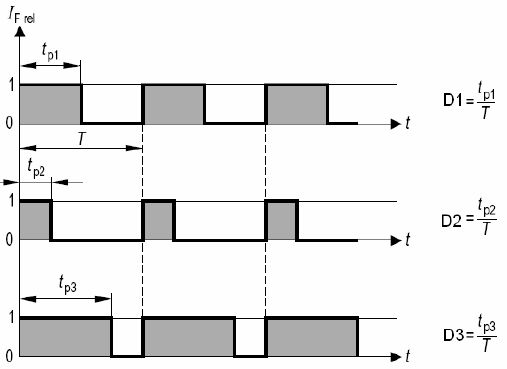
\includegraphics[bb=0 0 507 396]{led_pwm.png}}
	\caption{Управление яркосьтю светодиода ШИМ}
	\label{img:led_pwm}
\end{figure}

\begin{par}
При неизменном токе яркость свечения зависит от скважности
следующим образом: \\
    $$ D_2 < D_1 < D_3 $$

При этом, визуальная сила света будет меняться линейно при соответствующем
линейгном изменении скважности [TODO: откуда я взял эту информацию].
\end{par}

[TODO: А так же какова будет зависимость в чиселках]



%\newpage
%\begin{ thebibliography }{99}
%\bibitem{1} Автор1~И.~О. , Автор2~И.~О. Название первой книги. "−−− М.: Название	первого	издательства ,	1999.	"−−−	543~с .
%\bibitem{2} Автор3~И.~О. , Автор4~И.~О. Название второй книги. "−−− К.: Название	второго	издательства ,	1999.	"−−−	543~с .
%\end{ thebibliography }

%\ESKDappendix{рекомендуемое}{Исходный код этого документа} \ lstset {columns=fixed , language=[LaTeX]TeX,
%% basicstyle=\small , breaklines=true } \ l s t i n p u t l i s t i n g { general . tex }

\end{document}
